%% This style is provided for the ICSE 2015 main conference,
%% ICSE 2015 co-located events, and ICSE 2015 workshops.

%% bare_conf_ICSE15.tex
%% V1.4
%% 2014/05/22


%% This is a skeleton file demonstrating the use of IEEEtran.cls
%% (requires IEEEtran.cls version 1.7 or later) with an IEEE conference paper.
%%
%% Support sites:
%% http://www.michaelshell.org/tex/ieeetran/
%% http://www.ctan.org/tex-archive/macros/latex/contrib/IEEEtran/
%% and
%% http://www.ieee.org/

%%*************************************************************************
%% Legal Notice:
%% This code is offered as-is without any warranty either expressed or
%% implied; without even the implied warranty of MERCHANTABILITY or
%% FITNESS FOR A PARTICULAR PURPOSE!
%% User assumes all risk.
%% In no event shall IEEE or any contributor to this code be liable for
%% any damages or losses, including, but not limited to, incidental,
%% consequential, or any other damages, resulting from the use or misuse
%% of any information contained here.
%%
%% All comments are the opinions of their respective authors and are not
%% necessarily endorsed by the IEEE.
%%
%% This work is distributed under the LaTeX Project Public License (LPPL)
%% ( http://www.latex-project.org/ ) version 1.3, and may be freely used,
%% distributed and modified. A copy of the LPPL, version 1.3, is included
%% in the base LaTeX documentation of all distributions of LaTeX released
%% 2003/12/01 or later.
%% Retain all contribution notices and credits.
%% ** Modified files should be clearly indicated as such, including  **
%% ** renaming them and changing author support contact information. **
%%
%% File list of work: IEEEtran.cls, IEEEtran_HOWTO.pdf, bare_adv.tex,
%%                    bare_conf.tex, bare_jrnl.tex, bare_jrnl_compsoc.tex
%%*************************************************************************

% *** Authors should verify (and, if needed, correct) their LaTeX system  ***
% *** with the testflow diagnostic prior to trusting their LaTeX platform ***
% *** with production work. IEEE's font choices can trigger bugs that do  ***
% *** not appear when using other class files.                            ***
% The testflow support page is at:
% http://www.michaelshell.org/tex/testflow/



% Note that the a4paper option is mainly intended so that authors in
% countries using A4 can easily print to A4 and see how their papers will
% look in print - the typesetting of the document will not typically be
% affected with changes in paper size (but the bottom and side margins will).
% Use the testflow package mentioned above to verify correct handling of
% both paper sizes by the user's LaTeX system.
%
% Also note that the "draftcls" or "draftclsnofoot", not "draft", option
% should be used if it is desired that the figures are to be displayed in
% draft mode.
%
\documentclass[conference]{IEEEtran}
%
% If IEEEtran.cls has not been installed into the LaTeX system files,
% manually specify the path to it like:
% \documentclass[conference]{../sty/IEEEtran}





% Some very useful LaTeX packages include:
% (uncomment the ones you want to load)


% *** MISC UTILITY PACKAGES ***
%
%\usepackage{ifpdf}
% Heiko Oberdiek's ifpdf.sty is very useful if you need conditional
% compilation based on whether the output is pdf or dvi.
% usage:
% \ifpdf
%   % pdf code
% \else
%   % dvi code
% \fi
% The latest version of ifpdf.sty can be obtained from:
% http://www.ctan.org/tex-archive/macros/latex/contrib/oberdiek/
% Also, note that IEEEtran.cls V1.7 and later provides a builtin
% \ifCLASSINFOpdf conditional that works the same way.
% When switching from latex to pdflatex and vice-versa, the compiler may
% have to be run twice to clear warning/error messages.






% *** CITATION PACKAGES ***
%
%\usepackage{cite}
% cite.sty was written by Donald Arseneau
% V1.6 and later of IEEEtran pre-defines the format of the cite.sty package
% \cite{} output to follow that of IEEE. Loading the cite package will
% result in citation numbers being automatically sorted and properly
% "compressed/ranged". e.g., [1], [9], [2], [7], [5], [6] without using
% cite.sty will become [1], [2], [5]--[7], [9] using cite.sty. cite.sty's
% \cite will automatically add leading space, if needed. Use cite.sty's
% noadjust option (cite.sty V3.8 and later) if you want to turn this off.
% cite.sty is already installed on most LaTeX systems. Be sure and use
% version 4.0 (2003-05-27) and later if using hyperref.sty. cite.sty does
% not currently provide for hyperlinked citations.
% The latest version can be obtained at:
% http://www.ctan.org/tex-archive/macros/latex/contrib/cite/
% The documentation is contained in the cite.sty file itself.





% *** GRAPHICS RELATED PACKAGES ***
%
\ifCLASSINFOpdf
  % \usepackage[pdftex]{graphicx}
  % declare the path(s) where your graphic files are
  % \graphicspath{{../pdf/}{../jpeg/}}
  % and their extensions so you won't have to specify these with
  % every instance of \includegraphics
  % \DeclareGraphicsExtensions{.pdf,.jpeg,.png}
\else
  % or other class option (dvipsone, dvipdf, if not using dvips). graphicx
  % will default to the driver specified in the system graphics.cfg if no
  % driver is specified.
  % \usepackage[dvips]{graphicx}
  % declare the path(s) where your graphic files are
  % \graphicspath{{../eps/}}
  % and their extensions so you won't have to specify these with
  % every instance of \includegraphics
  % \DeclareGraphicsExtensions{.eps}
\fi
% graphicx was written by David Carlisle and Sebastian Rahtz. It is
% required if you want graphics, photos, etc. graphicx.sty is already
% installed on most LaTeX systems. The latest version and documentation can
% be obtained at:
% http://www.ctan.org/tex-archive/macros/latex/required/graphics/
% Another good source of documentation is "Using Imported Graphics in
% LaTeX2e" by Keith Reckdahl which can be found as epslatex.ps or
% epslatex.pdf at: http://www.ctan.org/tex-archive/info/
%
% latex, and pdflatex in dvi mode, support graphics in encapsulated
% postscript (.eps) format. pdflatex in pdf mode supports graphics
% in .pdf, .jpeg, .png and .mps (metapost) formats. Users should ensure
% that all non-photo figures use a vector format (.eps, .pdf, .mps) and
% not a bitmapped formats (.jpeg, .png). IEEE frowns on bitmapped formats
% which can result in "jaggedy"/blurry rendering of lines and letters as
% well as large increases in file sizes.
%
% You can find documentation about the pdfTeX application at:
% http://www.tug.org/applications/pdftex





% *** MATH PACKAGES ***
%
%\usepackage[cmex10]{amsmath}
% A popular package from the American Mathematical Society that provides
% many useful and powerful commands for dealing with mathematics. If using
% it, be sure to load this package with the cmex10 option to ensure that
% only type 1 fonts will utilized at all point sizes. Without this option,
% it is possible that some math symbols, particularly those within
% footnotes, will be rendered in bitmap form which will result in a
% document that can not be IEEE Xplore compliant!
%
% Also, note that the amsmath package sets \interdisplaylinepenalty to 10000
% thus preventing page breaks from occurring within multiline equations. Use:
%\interdisplaylinepenalty=2500
% after loading amsmath to restore such page breaks as IEEEtran.cls normally
% does. amsmath.sty is already installed on most LaTeX systems. The latest
% version and documentation can be obtained at:
% http://www.ctan.org/tex-archive/macros/latex/required/amslatex/math/





% *** SPECIALIZED LIST PACKAGES ***
%
%\usepackage{algorithmic}
% algorithmic.sty was written by Peter Williams and Rogerio Brito.
% This package provides an algorithmic environment fo describing algorithms.
% You can use the algorithmic environment in-text or within a figure
% environment to provide for a floating algorithm. Do NOT use the algorithm
% floating environment provided by algorithm.sty (by the same authors) or
% algorithm2e.sty (by Christophe Fiorio) as IEEE does not use dedicated
% algorithm float types and packages that provide these will not provide
% correct IEEE style captions. The latest version and documentation of
% algorithmic.sty can be obtained at:
% http://www.ctan.org/tex-archive/macros/latex/contrib/algorithms/
% There is also a support site at:
% http://algorithms.berlios.de/index.html
% Also of interest may be the (relatively newer and more customizable)
% algorithmicx.sty package by Szasz Janos:
% http://www.ctan.org/tex-archive/macros/latex/contrib/algorithmicx/




% *** ALIGNMENT PACKAGES ***
%
%\usepackage{array}
% Frank Mittelbach's and David Carlisle's array.sty patches and improves
% the standard LaTeX2e array and tabular environments to provide better
% appearance and additional user controls. As the default LaTeX2e table
% generation code is lacking to the point of almost being broken with
% respect to the quality of the end results, all users are strongly
% advised to use an enhanced (at the very least that provided by array.sty)
% set of table tools. array.sty is already installed on most systems. The
% latest version and documentation can be obtained at:
% http://www.ctan.org/tex-archive/macros/latex/required/tools/


%\usepackage{mdwmath}
%\usepackage{mdwtab}
% Also highly recommended is Mark Wooding's extremely powerful MDW tools,
% especially mdwmath.sty and mdwtab.sty which are used to format equations
% and tables, respectively. The MDWtools set is already installed on most
% LaTeX systems. The lastest version and documentation is available at:
% http://www.ctan.org/tex-archive/macros/latex/contrib/mdwtools/


% IEEEtran contains the IEEEeqnarray family of commands that can be used to
% generate multiline equations as well as matrices, tables, etc., of high
% quality.


%\usepackage{eqparbox}
% Also of notable interest is Scott Pakin's eqparbox package for creating
% (automatically sized) equal width boxes - aka "natural width parboxes".
% Available at:
% http://www.ctan.org/tex-archive/macros/latex/contrib/eqparbox/





% *** SUBFIGURE PACKAGES ***
%\usepackage[tight,footnotesize]{subfigure}
% subfigure.sty was written by Steven Douglas Cochran. This package makes it
% easy to put subfigures in your figures. e.g., "Figure 1a and 1b". For IEEE
% work, it is a good idea to load it with the tight package option to reduce
% the amount of white space around the subfigures. subfigure.sty is already
% installed on most LaTeX systems. The latest version and documentation can
% be obtained at:
% http://www.ctan.org/tex-archive/obsolete/macros/latex/contrib/subfigure/
% subfigure.sty has been superceeded by subfig.sty.



%\usepackage[caption=false]{caption}
%\usepackage[font=footnotesize]{subfig}
% subfig.sty, also written by Steven Douglas Cochran, is the modern
% replacement for subfigure.sty. However, subfig.sty requires and
% automatically loads Axel Sommerfeldt's caption.sty which will override
% IEEEtran.cls handling of captions and this will result in nonIEEE style
% figure/table captions. To prevent this problem, be sure and preload
% caption.sty with its "caption=false" package option. This is will preserve
% IEEEtran.cls handing of captions. Version 1.3 (2005/06/28) and later
% (recommended due to many improvements over 1.2) of subfig.sty supports
% the caption=false option directly:
%\usepackage[caption=false,font=footnotesize]{subfig}
%
% The latest version and documentation can be obtained at:
% http://www.ctan.org/tex-archive/macros/latex/contrib/subfig/
% The latest version and documentation of caption.sty can be obtained at:
% http://www.ctan.org/tex-archive/macros/latex/contrib/caption/




% *** FLOAT PACKAGES ***
%
%\usepackage{fixltx2e}
% fixltx2e, the successor to the earlier fix2col.sty, was written by
% Frank Mittelbach and David Carlisle. This package corrects a few problems
% in the LaTeX2e kernel, the most notable of which is that in current
% LaTeX2e releases, the ordering of single and double column floats is not
% guaranteed to be preserved. Thus, an unpatched LaTeX2e can allow a
% single column figure to be placed prior to an earlier double column
% figure. The latest version and documentation can be found at:
% http://www.ctan.org/tex-archive/macros/latex/base/



%\usepackage{stfloats}
% stfloats.sty was written by Sigitas Tolusis. This package gives LaTeX2e
% the ability to do double column floats at the bottom of the page as well
% as the top. (e.g., "\begin{figure*}[!b]" is not normally possible in
% LaTeX2e). It also provides a command:
%\fnbelowfloat
% to enable the placement of footnotes below bottom floats (the standard
% LaTeX2e kernel puts them above bottom floats). This is an invasive package
% which rewrites many portions of the LaTeX2e float routines. It may not work
% with other packages that modify the LaTeX2e float routines. The latest
% version and documentation can be obtained at:
% http://www.ctan.org/tex-archive/macros/latex/contrib/sttools/
% Documentation is contained in the stfloats.sty comments as well as in the
% presfull.pdf file. Do not use the stfloats baselinefloat ability as IEEE
% does not allow \baselineskip to stretch. Authors submitting work to the
% IEEE should note that IEEE rarely uses double column equations and
% that authors should try to avoid such use. Do not be tempted to use the
% cuted.sty or midfloat.sty packages (also by Sigitas Tolusis) as IEEE does
% not format its papers in such ways.





% *** PDF, URL AND HYPERLINK PACKAGES ***
%
%\usepackage{url}
% url.sty was written by Donald Arseneau. It provides better support for
% handling and breaking URLs. url.sty is already installed on most LaTeX
% systems. The latest version can be obtained at:
% http://www.ctan.org/tex-archive/macros/latex/contrib/misc/
% Read the url.sty source comments for usage information. Basically,
% \url{my_url_here}.





% *** Do not adjust lengths that control margins, column widths, etc. ***
% *** Do not use packages that alter fonts (such as pslatex).         ***
% There should be no need to do such things with IEEEtran.cls V1.6 and later.
% (Unless specifically asked to do so by the journal or conference you plan
% to submit to, of course. )

%\usepackage{placeins}
% correct bad hyphenation here
\hyphenation{op-tical net-works semi-conduc-tor}
\usepackage[linesnumbered,ruled,vlined]{algorithm2e}
\usepackage[pdftex]{graphicx} 
%\usepackage{stfloats}
\usepackage{cite}
\usepackage[cmex10]{amsmath}
\usepackage{algorithmic}
\usepackage{multirow}
%\fnbelowfloat
\usepackage[tight,footnotesize]{subfigure}
\usepackage{listings}
\usepackage{color}
\usepackage{url}
\definecolor{dkgreen}{rgb}{0,0.6,0}
\definecolor{gray}{rgb}{0.5,0.5,0.5}
\definecolor{mauve}{rgb}{0.58,0,0.82}
\usepackage{multirow}
\usepackage{booktabs}

\usepackage{amssymb}
\lstset{frame=tb,
	language=Java,
	aboveskip=3mm,
	belowskip=3mm,
	showstringspaces=false,
	columns=flexible,
	basicstyle={\small\ttfamily},
	numbers=none,
	numberstyle=\tiny\color{gray},
	keywordstyle=\color{blue},
	commentstyle=\color{dkgreen},
	stringstyle=\color{mauve},
	tabsize=3
}
 %\usepackage{titlesec}

\setcounter{topnumber}{10}
\setcounter{bottomnumber}{10}
\setcounter{totalnumber}{10}
\renewcommand{\floatpagefraction}{.9}
\renewcommand{\textfraction}{.2}
\DeclareGraphicsExtensions{.pdf,.png,.jpg,.mps} 
\begin{document}
%
% paper title
% can use linebreaks \\ within to get better formatting as desired
\title{GENECO: A Generic Framework for Non-functional Testing of Code Generators}


% author names and affiliations
% use a multiple column layout for up to three different
% affiliations
%\author{\IEEEauthorblockN{Michael Shell}
%\IEEEauthorblockA{School of Electrical and\\Computer Engineering\\
%Georgia Institute of Technology\\
%Atlanta, Georgia 30332--0250\\
%Email: http://www.michaelshell.org/contact.html}
%\and
%\IEEEauthorblockN{Homer Simpson}
%\IEEEauthorblockA{Twentieth Century Fox\\
%Springfield, USA\\
%Email: homer@thesimpsons.com}
%\and
%\IEEEauthorblockN{James Kirk\\ and Montgomery Scott}
%\IEEEauthorblockA{Starfleet Academy\\
%San Francisco, California 96678-2391\\
%Telephone: (800) 555--1212\\
%Fax: (888) 555--1212}}

% conference papers do not typically use \thanks and this command
% is locked out in conference mode. If really needed, such as for
% the acknowledgment of grants, issue a \IEEEoverridecommandlockouts
% after \documentclass

% for over three affiliations, or if they all won't fit within the width
% of the page, use this alternative format:
%
%\author{\IEEEauthorblockN{Mohamed Boussaa\IEEEauthorrefmark{1},
%Olivier Barais\IEEEauthorrefmark{2},
%Gerson Sunye\IEEEauthorrefmark{1},
%and Benoit Baudry\IEEEauthorrefmark{1} }
%\IEEEauthorblockA{\IEEEauthorrefmark{1}Inria / IRISA, University of Rennes 1, France\\
%	Email: \IEEEauthorrefmark{1}mohamed.boussaa@inria.fr,
%	\IEEEauthorrefmark{1}olivier.barais@irisa.fr,
%	\IEEEauthorrefmark{1}gerson.sunye@inria.fr,
%	\IEEEauthorrefmark{1}benoit.baudry@inria.fr}	
%}
\author{\IEEEauthorblockN{Mohamed Boussaa, Olivier Barais, Gerson Suny\'e, and Benoit Baudry}
\IEEEauthorblockA{
	Inria/IRISA Rennes, France\\
Email: \{mohamed.boussaa, olivier.barais, gerson.sunye, benoit.baudry\}@inria.fr
}}



% use for special paper notices
%\IEEEspecialpapernotice{(Invited Paper)}

\newcommand{\etal}{et al.}
\newcommand{\eg}[0]{e.\,g.}
\newcommand{\ie}[0]{i.\,e.}


% make the title area
\maketitle


\begin{abstract}

Generally, compiler users apply different optimizations to generate efficient code with respect to non-functional properties such as memory consumption, execution time, among others. However, due to the huge number of optimizations provided by modern compilers, finding the best optimization sequence for a specific objective and a given program is more and more challenging. 

This paper proposes NOTICE, a component-based framework for non-functional testing of compilers through the monitoring of generated code in a controlled sand-boxing environment.
We evaluate the effectiveness of our approach by verifying the optimizations performed by GCC compiler.
Our experimental results show that our approach is able to auto-tune compilers according to user requirements and construct optimizations that yield to better performance results than standard optimization levels.
We also demonstrate that NOTICE can be used to automatically construct optimization levels that represent optimal trade-offs between multiple non-functional properties such as execution time and resource usage requirements.


%Compiler users tend to improve software programs in a safe and profitable way.
%Generally, they can apply different optimizations to generate efficient code with respect to non-functional properties such as memory consumption, execution time, code size, among others. However, due to the huge number of optimizations provided by modern compilers, finding the best optimization sequence for a specific objective and a given program is more and more challenging. 
%This paper proposes NOTICE, a component-based framework for non-functional testing of compilers through the monitoring of generated code in a controlled sand-boxing environment.
%NOTICE is an on-demand tool that employs different mono and multi-objective evolutionary search algorithms to construct optimization sequences that satisfy user key objectives (execution time, CPU or memory usage, etc.).
%In our approach, we focus on the relationship between runtime execution of optimized code and resource consumption profiles (CPU and memory usage) by providing a fine-grained understanding and analysis of compilers behavior regarding optimizations.
%We evaluate the effectiveness of our approach by verifying the optimizations performed by GCC compiler.
%Our experimental results show that our approach is able to auto-tune compilers and construct optimizations that yield to better performance results than standard optimization levels.
%We also demonstrate that NOTICE can be used to automatically construct optimization levels that represent optimal trade-offs between multiple non-functional properties, such as execution time and resource consumption metrics.



 



%they are highly dependent on target platforms
\end{abstract}
\smallskip
\noindent \textbf{Keywords.} \textit{software quality, non-functional properties, compilers, testing}.
% HD-Services will run within a heterogeneous and distributed infrastructure. To facilitate the testing of this kind of services, we need to deploy HD-services on an elastic infrastructure that provides preconfigured virtual server images, storage and network connectivity that may be provisioned by HD-Developers. Monitoring information should also be provided to inform about resource utilization required/needed and to automate the resource management. For this purpose, we propose a testing infrastructure based on docker environment. Docker will automate the deployment of applications inside software containers. It will simplify the creation of highly distributed systems by allowing multiple applications to run autonomously on a server (basically a cloud server). Docker will provide a platform as a service (PaaS) style of deployment for HD-Services. Consequently, we will rely on this technology and benefit from all its advantages to:
%1- Deploy preconfigured application to test within docker containers
%2- Automate test suites generation
%3- Monitor service containers
%4- Limit and manage resources for each running container
%5- Gather performance metrics (CPU, Memory, I/O, etc.)
%As a consequence, we are going to integrate a collection of docker technologies to define the adequate infrastructure for testing HD-Services.



%In model-driven engineering, developers use different code generators to translate source programs represented in a graphical modeling language into general purpose programming languages such as C, Java, C++,etc.  These code generators serve as a basis to target different ranges of platforms. Many technologies, such as Docker containers, provide new opportunities to automate the deployment of produced code into a distributed and heterogeneous component-based infrastructure. In fact, during the code generation process, different optimizations may be applied for code transformation. For example, embedded systems for which code is generated often have limited resources. Therefore, optimization techniques must be applied whenever possible to generate efficient code with respect to memory consumption, execution time, disk writing speed, among others. Sometimes, optimizations can even lead to memory leaks or execution bottlenecks especially for resource-constrained systems. So, to ensure the efficiency of generated code, deployed components must be checked and verified regarding their non-functional behavior. This paper describes a component-based tool for testing and monitoring generated code. It provides a fine-grained understanding of resource consumption and analysis of components behavior regarding optimizations. We evaluate the effectiveness of our test approach by means of testing optimizations performed by the GCC compiler, a widely used compiler in software engineering community. We present as well a number of case studies, in which the tool was successfully used.
\section{Introduction}
Compiler users tend to improve software programs in a safe and profitable way. Modern compilers provide a broad collection of optimizations that can be applied during the code generation process. 
For functional testing of compilers, software testers generally use to re-execute a set of test suites on different optimized software versions and compare the functional outcome that can be either pass (correct behaviour) or fail (incorrect behaviour, crashes or bugs)~\cite{chen2016empirical,hoste2008cole,le2014compiler}.

For non-functional testing, improvement of source code programs in term of performance can refer to several different non-functional properties of the produced code such as code size, resource or energy consumption, execution time, among others~\cite{almagor2004finding,pan2006fast}.
Testing non-functional properties is more challenging because compilers may have a huge number of potential optimization combinations, making it hard and time-consuming for software developers to find/construct the sequence of optimizations that satisfies user specific key objectives and criteria. It also requires a comprehensive understanding of the underlying system architecture, the target application and the available optimizations of the compiler.

In some cases, these optimizations may negatively decrease the quality of the software and deteriorate application performance over time~\cite{molyneaux2009art}. 
As a consequence, compiler creators usually define fixed and program-independent sequence optimizations, which are based on their experiences and heuristics. For example, in GCC, we can distinguish optimization levels from O1 to O3. Each optimization level involves a fixed list of compiler optimization options and provide different trade-offs in term of non-functional properties.
Nevertheless, there is no guarantee that these optimization levels will perform well on untested architectures or for unseen applications. 
Thus, it is necessary to detect possible issues caused by source code changes such as performance regressions and help users to validate optimizations that induce to performance improvement.
%Many technologies, such as Docker containers, provide new opportunities to automate the deployment of produced code into a distributed and heterogeneous component-based infrastructure

We note also that when trying to optimize software performance,
many non-functional properties and design constraints must be involved and satisfied simultaneously to better optimize code.
Most of previous works try to optimize a single criterion (usually the execution time)~\cite{ballal2015compiler,chen2012deconstructing,demertzi2011analyzing} and ignore other important non-functional properties, more precisely resource consumption properties such as memory or CPU usage, that must be taken into consideration and can be equally important in relation to the performance. Sometimes, improving program execution time can be so expensive at the expense of resource usage which may decrease system performance. For example, embedded systems for which code is generated often have limited resources. Thus, optimization techniques must be applied whenever possible to generate efficient code and improve performance (in term of execution time) with respect to available resources (in term of CPU or memory usage)~\cite{nagiub2013automatic}.
Therefore, it is important to construct optimization levels that represent multiple trade-offs between non-functional properties, enabling the software designer to choose among different optimal solutions which best suit the system specifications.



%In this context, compilers suppose a decisive factor in the optimization. Compilers
%currently offer a large number of optimization options. However, this capability
%is never fully exploited as it involves a comprehensive understanding of
%the underlying computer architecture, the target application and the operation
%of the compiler.

 

In this paper, we propose NOTICE (as NOn-functional TestIng of CompilErs), a component-based framework for non-functional testing of compilers through the monitoring of generated code in a controlled sand-boxing environment. Our approach is based on micro-services to automate the deployment and monitoring of different variants of optimized code. NOTICE is an on-demand tool that employs mono and multi-objective evolutionary search algorithms to construct optimization sequences that satisfy user key objectives (execution time, code size, compilation time, CPU or memory usage, etc.).
In this paper, we make the following contributions:
\begin{itemize}  
	
	
	
	\item The paper introduces a novel formulation of compiler optimizations exploration problem using Novelty Search~\cite{lehman2008exploiting}. We evaluate the effectiveness of our approach by verifying the optimizations performed by GCC compiler.
	Our experimental results show that NOTICE is able to auto-tune compilers according to user choices (heuristics, objectives, programs, etc.) and construct optimizations that yield to better performance results than standard optimization levels.
	% and, to the best of our knowledge, this is the first paper in the literature to %use Novelty Search to evaluate optimization sequences.
	
	\item We propose a micro-service infrastructure to ensure the deployment and monitoring of different variants of optimized code. In this paper, we focus more on the relationship between runtime execution of optimized code and resource consumption profiles (CPU and memory usage) by providing a fine-grained understanding and analysis of compilers behavior regarding optimizations.
	

	\item We also demonstrate that NOTICE can be used to automatically construct optimization levels that represent optimal trade-offs between multiple non-functional properties, such as execution time, memory usage, CPU consumption, etc.
\end{itemize}


 
%This to ensure the efficiency of generated code, deployed components must be checked and verified regarding their non-functional behavior
%\footnote{\url{https://www.docker.com}} 



The paper is organized as follows. Section II describes the motivation behind this work. A search-based technique for compiler optimizations exploration is presented in Section III. We present in Section IV our infrastructure for non-functional testing using micro-services. The evaluation and results of our experiments are discussed in Section V. Finally, related work, concluding remarks and future work are provided in Sections VI and VII.


%The difference between classical compilers like GCC, LLVM and code generators is that code generators are used only by few people comparing to famous compilers like GCC. Moreover, code generators face a high rate of changes and update versions due to new development needs. Hence, it becomes necessary to check the quality of produced code. This will help software maintainers to verify the correct functioning of code generators.  Among the most important properties to check, we distinguish the non functional properties.

%Like traditional compilers, code generators typically perform multiple passes over various intermediate forms during code transformation. Many rules may also be applied and that differs from one generator to another. These passes are complex and highly dependent on target platform architecture. 

 
 

  % \section{Motivations}
 %\section{Previous work}
%\section{Approach Overview}

\section{Motivation}
\subsection{Compilers Optimizations}
In the past, researchers have shown that the choice of optimization sequences may impact software performance~\cite{almagor2004finding,chen2012deconstructing}. 
As a consequence, software-performance optimization becomes a key objective for both, software industries and developers, which are often willing to pay additional costs to meet specific performance goals, especially for resource-constrained systems.

Universal and predefined sequences, \eg, O1 to O3 in GCC, may not always produce good performance results and may be highly dependent on the benchmark and the source code they have been tested on~\cite{almagor2004finding,hoste2008cole}.
Indeed, each one of these optimizations interacts with the code and in turn with all other optimizations in complicated ways. Similarly, code transformations can either create or eliminate opportunities for other transformations and it is quite difficult for users to predict the effectiveness of optimizations on their source code program.
As a result, most software engineering programmers that are not familiar with compiler optimizations find difficulties to select effective optimization sequences.

To explore the large optimization space, users have to evaluate the effect of optimizations and optimization combinations, for different target platforms (see Figure 1). 
Thus, finding the optimal optimization options for an input source code is a challenging, very hard, and time-consuming problem. 
Many approaches~\cite{hoste2008cole,zhong2009tuning,sandran2012genetic,martins2014exploration} have attempted to solve this optimization selection problem using techniques such as genetic algorithms, iterative compilation, etc.

%problem
It is important to notice that performing optimizations to source code can be so expensive at the expense of resource usage and may induce to compiler bugs or crashes. 
%With the increasing of resource usage, it is important to evaluate the compiler behavior. 
Indeed, in a resource-constrained environment and because of insufficient resources, compiler optimizations can even lead to memory leaks or execution crashes~\cite{yang2011finding}. 
Thus, a fine-grained understanding of resource consumption and analysis of compilers behavior regarding optimizations becomes necessary to ensure the efficiency of generated code.
\begin{figure}[h]
	\centering
	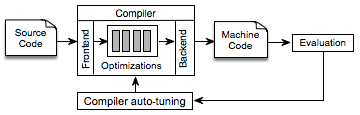
\includegraphics[width=1\hsize]{Ressources/autotuning.png}
	\caption{fig}
\end{figure}
\subsection{Example: GCC Compiler}

The GNU Compiler Collection, GCC, is a very popular collection of programming compilers, available for different platforms.
GCC exposes its various optimizations via a number of flags that can be turned on or off through command-line compiler switches. 
The diversity of available optimization options makes the design space for optimization level very huge, increasing the need for heuristics to explore the search space of feasible optimizations sequences.

% We choose GCC compiler as a motivating example in order to explain how we would study the impact of compiler optimizations using a component-based infrastructure for testing and monitoring.
% In next section, we present a search-based technique called Novelty Search for automatic generation of optimization sequences.

For instance, version 4.8.4 provides a wide range of command-line optimizations that can be enabled or disabled, including more than 150 options for optimization. 
Table I summarizes the optimization flags that are enabled by the default optimization levels O1 to O3.
%For example, in GCC, we can distinguish optimization levels from O1 to O3. Each optimization level involves a fixed list of compiler optimization options
We count 76 optimization flags, resulting in a huge space with $2^{76}$ possible optimization combinations.
In our approach, we did not consider some optimization options that are enabled by default, since they do not affect the performance of generated binaries.
Optimization flags in GCC can be turned off by using "fno-"+flag instead of "f"+flag in the beginning of each optimization. 
We use this technique to play with compiler switches.

\begin{table}
	\label{table:options}
	\centering
	\caption{Compiler optimization options within standard optimization levels}
	\scalebox{0.88}{
		\begin{tabular}[c]{|c|p{3cm}||c|p{3cm}|}
			
			
			\cline{1-4}
			Level & Optimization option & Level & Optimization option  \\
			\hline
			O1 & 
			-fauto-inc-dec \newline
			-fcompare-elim \newline
			-fcprop-registers \newline
			-fdce \newline
			-fdefer-pop \newline
			-fdelayed-branch \newline
			-fdse \newline
			-fguess-branch-probability \newline
			-fif-conversion2 \newline
			-fif-conversion \newline
			-fipa-pure-const \newline
			-fipa-profile \newline
			-fipa-reference\newline 
			-fmerge-constants\newline
			-fsplit-wide-types \newline
			-ftree-bit-ccp \newline
			-ftree-builtin-call-dce \newline
			-ftree-ccp \newline
			-ftree-ch \newline
			-ftree-copyrename \newline
			-ftree-dce \newline
			-ftree-dominator-opts \newline
			-ftree-dse \newline
			-ftree-forwprop \newline
			-ftree-fre \newline
			-ftree-phiprop \newline
			-ftree-slsr \newline
			-ftree-sra \newline
			-ftree-pta \newline
			-ftree-ter \newline
			-funit-at-a-time
			
			&
			\multirow{2}{*}{O2} & \multirow{2}{6cm} {
				-fthread-jumps\newline 
				-falign-functions\newline  
				-falign-jumps \newline
				-falign-loops  \newline
				-falign-labels \newline
				-fcaller-saves \newline
				-fcrossjumping \newline
				-fcse-follow-jumps  \newline
				-fcse-skip-blocks \newline
				-fdelete-null-pointer-checks \newline
				-fdevirtualize \newline
				-fexpensive-optimizations \newline
				-fgcse  \newline
				-fgcse-lm  \newline
				-fhoist-adjacent-loads \newline
				-finline-small-functions \newline
				-findirect-inlining \newline
				-fipa-sra \newline
				-foptimize-sibling-calls \newline
				-fpartial-inlining \newline
				-fpeephole2 \newline
				-fregmove \newline
				-freorder-blocks  \newline
				-freorder-functions \newline
				-frerun-cse-after-loop \newline 
				-fsched-interblock \newline 
				-fsched-spec \newline
				-fschedule-insns  \newline
				-fschedule-insns2 \newline
				-fstrict-aliasing \newline
				-fstrict-overflow \newline
				-ftree-switch-conversion\newline -ftree-tail-merge \newline
				-ftree-pre \newline
				-ftree-vrp
			} \\
			\cline{1-2}
			O3 & 
			-finline-functions \newline
			-funswitch-loops\newline
			-fpredictive-commoning \newline
			-fgcse-after-reload \newline
			-ftree-vectorize \newline
			-fvect-cost-model \newline
			-ftree-partial-pre \newline 
			-fipa-cp-clone  & &  \\
			\cline{1-2}
			Ofast & -ffast-math &   &  \\
			\hline
			
		\end{tabular}
	}
\end{table}
\section{Evolutionary Exploration of Compiler Optimizations }


Many techniques (meta-heuristics, constraint programming, etc.) can be used to explore the large set of optimization combinations of modern compilers. 
In our approach, we study the use of the Novelty Search (NS) technique to identify the set of compiler optimization options that optimize the non-functional properties of code.

\subsection{Novelty Search Adaptation}
%Optimization options are difficult and even impossible to be chosen by programmers or compiler users.
%Therefore, a tool to help users to choose the best set of options becomes necessary to achieve a compiler optimization with effectiveness.

In this work, we aim at providing a new alternative for choosing effective compiler optimization options compared to the state of the art approaches. 
In fact, since the search space of possible combinations is too large, we aim at using a new search-based technique called Novelty Search~\cite{lehman2008exploiting} to tackle this issue. 
The idea of this technique is to explore the search space of possible compiler flag options by considering sequence diversity as a single objective. 
Instead of having a fitness-based selection that maximizes one of the non-functional objectives, we select optimization sequences based on a novelty score showing how different they are compared to all other combinations evaluated so far. 
We claim that the search towards effective optimization sequences is not straightforward since the interactions between optimizations is too complex and difficult to define. 
For instance, in a previous work~\cite{chen2012deconstructing}, Chen et al. showed that handful optimizations may lead to higher performance than other techniques of iterative optimization. 
In fact, the fitness-based search may be trapped into some local optima that cannot escape. 
This phenomenon is known as \textit{"diversity loss"}. For example, if the most effective optimization sequence that induces less execution time lies far from the search space defined by the gradient of the fitness function, then some promising search areas may not be reached. 
The issue of premature convergence to local optima has been a common problem in evolutionary algorithms. 
Many methods are proposed to overcome this problem~\cite{banzhaf1996effect}. 
However, all these efforts use a fitness-based selection to guide the search. Considering diversity as the unique objective function to be optimized may be a key solution to this problem.
Therefore, during the evolutionary process, we select optimization sequences that remain in sparse regions of the search space in order to guide the search towards novelty. 
In the meantime, we choose to gather non-functional metrics of explored sequences such as memory consumption. 
We describe in more details the way we are collecting these non-functional metrics in section 4.

Generally, NS acts like GAs (Example of GA use in  \cite{cooper2002adaptive}). However, NS needs extra changes. First, a new novelty metric is required to replace the fitness function. Then, an archive must be added to the algorithm, which is a kind of a database that remembers individuals that were highly novel when they were discovered in past generations. 
Algorithm~\ref{algo:search} describes the overall idea of our NS adaptation. The algorithm takes as input a source code program and a list of optimizations. We initialize first the novelty parameters and create a new archive with limit size L (lines 1 \& 2). In this example, we gather information about memory consumption. In lines 3 \& 4, we compile and execute the input program without any optimization (O0). Then, we measure the resulting memory consumption. By doing so, we will be able to compare it to the memory consumption of new generated solutions. The best solution is the one that yields to the lowest memory consumption compared to O0 usage.
Before starting the evolutionary process, we generate an initial population with random sequences. Line 6-21 encode the main NS loop, which searches for the best sequence in terms of memory consumption. For each sequence in the population, we compile the input program, execute it and evaluate the solution by calculating the average distance from its k-nearest neighbors. Sequences that get a novelty metric higher than the novelty threshold T are added to the archive. T defines the threshold for how novel a sequence has to be before it is added to the archive. In the meantime, we check if the optimization sequence yields to the lowest memory consumption so that, we can consider it as the best solution. Finally, genetic operators
(mutation and crossover) are applied afterwards to fulfill the next population. This process is iterated until reaching the maximum number of evaluations.


\begin{algorithm}
\algsetup{linenosize=\tiny}
  \footnotesize
  %footnotesize
	\caption{Novelty search algorithm for compiler optimization exploration}
	\label{algo:search}
	\begin{algorithmic}[1]
	
		\REQUIRE Optimization options $\mathcal{O}$
		\REQUIRE Program $\mathcal{C}$
		\REQUIRE Novelty threshold $\mathcal{T}$
		\REQUIRE Limit $\mathcal{L}$
		\REQUIRE Nearest neighbors $\mathcal{K}$
		\REQUIRE Number of evaluations $\mathcal{N}$
		\ENSURE Best optimization sequence $best\_sequence$
		\STATE $initialize\_parameters(\mathcal{L},\mathcal{T},\mathcal{N},\mathcal{K})$
		\STATE $create\_archive(\mathcal{L})$
		\STATE 	$generated\_code \gets compile(\textit{"-O0"},\mathcal{C})$
		\STATE 	$minimum\_usage \gets execute(generated\_code)$
		\STATE $population \gets random\_sequences(\mathcal{O})$
		\REPEAT
		\FOR{$sequence \in population$}   
		\STATE 	$generated\_code \gets compile(sequence,\mathcal{C})$
		\STATE 	$memory\_usage \gets execute(generated\_code)$
		\STATE	$novelty\_metric(sequence) \gets distFromKnearest(archive,population,\mathcal{K})$
		\IF{$novelty\_metric > \mathcal{T}$}
		\STATE	$archive \gets archive \cup sequence$
		\ENDIF
		
			\IF{$memory\_usage < minimum\_usage$}
			\STATE	$best\_sequence \gets sequence$
			\STATE	$minimum\_usage \gets memory\_usage$
			\ENDIF
			
		\ENDFOR
		\STATE		$new\_population \gets generate\_new\_population(population)$
		\STATE		$generation \gets generation + 1$
		\UNTIL{$generation = \mathcal{N}$}
		\RETURN $best\_sequence$
	\end{algorithmic}
\end{algorithm}


\subsubsection{Optimization Sequence Representation}
For our case study, a candidate solution represents all compiler switches that are used in the four standard optimization levels (O1, O2, O3 and Ofast). Thereby, we represent this solution as a vector where each dimension is a compiler flag. 
The variables that represent compiler options are represented as genes in a chromosome. 
Thus, a solution represents the CFLAGS value used by GCC to compile programs.
A solution has always the same size, which corresponds to the total number of involved flags. 
However, during the evolutionary process, these flags are turned on or off depending on the mutation and crossover operators (see example in Figure 2). As well, we keep the same order of invoking compiler flags since that does not affect the optimization process and it is handled internally by GCC.
\begin{figure}[h]
	\centering
	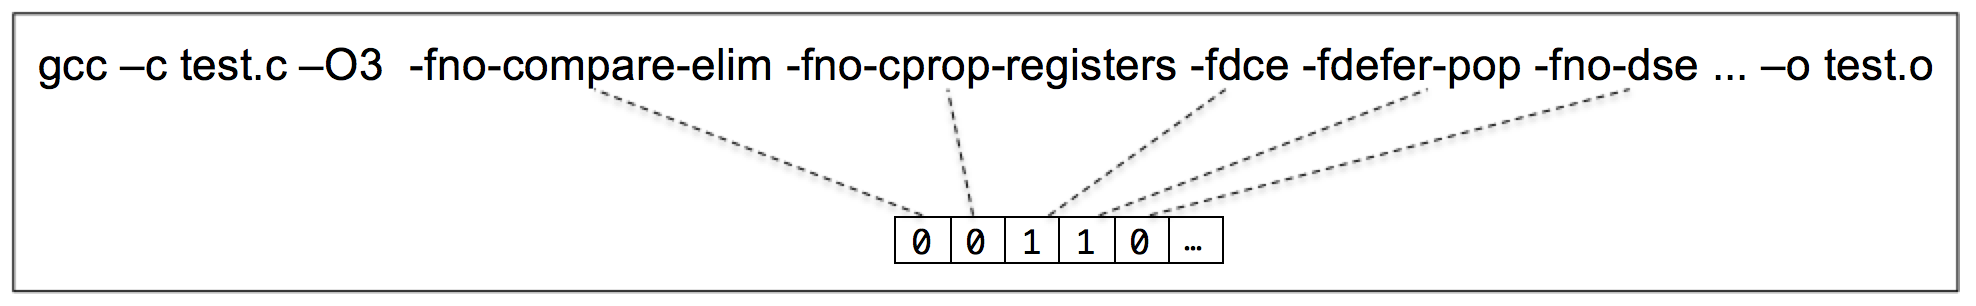
\includegraphics[width=1\hsize]{Ressources/individual.png}
	\caption{Solution representation}
	
\end{figure}

\subsubsection{Novelty Metric}
The Novelty metric expresses the sparseness of an input optimization sequence. It measures its distance to all other sequences in the current population and to all sequences that were discovered in the past (\ie, sequences in the archive). 
We can quantify the sparseness of a solution as the average distance to the k-nearest neighbors. 
If the average distance to a given point's nearest neighbors is large then it belongs to a sparse area and will get a high novelty score. 
Otherwise, if the average distance is small so it belongs certainly to a dense region then it will get a low novelty score. 
The distance between two sequences is computed as the total number of symmetric differences among optimization sequences. Formally, we define this distance as follows :
\begin{equation}
distance(S1,S2)=\left | S1 \bigtriangleup S2 \right |
\end{equation}
where $S1$ and $S2$ are two selected optimization sequences (solutions). The distance value is equal to 0 if the two optimization sequences are similar and higher than 0 if there is at least one optimization difference. The maximum distance value is equal to the total number of input flags.

To measure the sparseness of a solution, we use the previously defined distance to compute the average distance of a sequence to its k-nearest neighbors. In this context, we define the novelty metric of a particular solution as follows:
\begin{equation}
NM(S) = \frac{1}{k} \sum_{i=1}^{k} distance(S,\mu _{i})
\end{equation}
where $\mu _{i}$ is the $i^{th}$ nearest neighbor of the solution S within the population and the archive of novel individuals. 

\subsection{Novelty Search For Multi-objective Optimization}
A multi-objective approach provides a trade-off between two objectives where the developers can select their desired solution from the Pareto-optimal front. The idea of this approach is to use multi-objective algorithms to find trade-offs between non-functional properties of generated code such as \textit{$<$ExecutionTime--MemoryUsage$>$}. The correlations we are trying to investigate are more related to the trade-offs between resource consumption and execution time.
  
For instance, NS can be easily adapted to multi-objective problems. In this adaptation, the SBSE formulation remains the same as described in Algorithm 1. However, in order to evaluate the new discovered solutions, we have to consider two main objectives and add the non-dominated solutions to the Pareto non-dominated set. We apply the Pareto dominance relation to find solutions that are not Pareto dominated by any other solution discovered so far, like in NSGA-II~\cite{lokuciejewski2010multi, deb2002fast}. Then, this Pareto non-dominated set is returned as a result.
There is typically more than one optimal solution at the end of NS. The maximum size of the final Pareto set cannot exceed the size of the initial population.

\section{An Infrastructure for Non-functional Testing Using System Containers}

In general, there are many non-functional properties that can be influenced by compiler optimizations, \eg, reliability, performance (response time), quality, etc. In this paper, we focus on the efficiency of optimized code in term of resource consumption (memory and CPU).
Therefore, we need to deploy the test harness, \ie the produced binaries, on an elastic infrastructure that provides compilers users facilities to ensure the deployment and monitoring of different variants of optimized code. 
%Monitoring information should also be provided to inform about resource utilization required/needed and to automate the resource management of deployed components. 
For this purpose, we propose NOTICE, a non-functional testing infrastructure based on System Container techniques such as Docker\footnote{\url{https://www.docker.com}} environment. 

%Docker will automate the deployment and execution of applications inside software containers by allowing multiple applications to run autonomously on a server (basically a cloud server). 
%It provides a platform as a service (PaaS) style of deployment for software programs. 
Consequently, we rely on this technology and benefit from all its advantages to:
\begin{enumerate}
	\item Deploy generated code within Docker containers
	\item Automate optimization sequences generation
	\item Execute and monitor service containers
	\item Gather performance metrics (CPU, Memory, I/O, etc.)
\end{enumerate}

%We integrate a collection of containers to define the adequate infrastructure for testing and monitoring of compilers. 


\subsection{System Containers as Deployment Environment}
Before starting to monitor and test generated code, we have to describe the deployment environment of NOTICE.

We aim to use Docker Linux containers to monitor the execution of produced binaries by GCC compilers in term of resource usage. 
To do so, we use Docker, an open source engine that automates the deployment of any application as a lightweight, portable, and self-sufficient container that runs virtually on a host machine. 
%To achieve that, Docker uses the Linux container technology. 
Using Docker, we can define preconfigured applications and servers to host. We can also define the way the service should be deployed in the host machine. 
As properties, we can define the OS where the service has to run, dependencies, etc. Once Docker images are defined, we can instantiate different containers.
A simple way to define Docker images is to use Dockerfiles. Docker can build images automatically by reading the instructions from a Dockerfile. 
Therefore, for our experiments we describe a Dockerfile that defines the target compiler to test, as well the container OS. The same Docker image will be used then, to execute different instances of generated code. We use Docker Hub\footnote{https://hub.docker.com/} for building, saving, and managing all our Docker images. It represents a cloud-based registry service for building and shipping application or service containers.

Basically, each container deploys an optimized version of the input source code program.

Docker uses as well Linux control groups (cgroups) to group processes running in the container. This allows us to manage the resources of a group of processes, which is very valuable. 
This approach increases the flexibility when we want to manage resources, since we can manage every group individually. 

Therefore, to run our experiments, each optimized program is executed individually inside an isolated Linux container. By doing so, we ensure that each executed program runs in isolation without being affected by the host machine or any other processes. Moreover, since a container is cheap to create, we are able to create too many containers as long as we have new programs to execute. 

Since each program execution requires a new container to be created, it is crucial to remove and kill containers that have finished their job to eliminate the load on the system. In fact, containers/programs are running sequentially without defining any constraints on resource utilization for each container. So once execution is done, resources reserved for the container are automatically released to enable spawning next containers. Therefore, the host machine will not suffer too much from the performance trade-offs.



Using Linux containers, we offer facilities to compilers users to test  
The main advantages that Docker offers compared to using a full stack virtualization solution is less performance overhead and resource isolation.
\subsection{Runtime Testing Components}
In order to test our running applications within Docker containers, we aim to use a set of Docker components to ease the extraction of non-functional properties.
\subsubsection{Monitoring Component}
This container will provide us an understanding of the resource usage and performance characteristics of our running containers. Generally, Docker containers rely on cgroups file systems to expose a lot of metrics about accumulated CPU cycles, memory, block I/O usage, etc. Therefore, our monitoring component automates the extraction of runtime performance metrics using cgroups. For example, we access to live resource consumption of each container available at the cgroup file system via stats found in $/sys/fs/cgroup/cpu/docker/(longid)/$ (for CPU consumption) and $/sys/fs/cgroup/memory/docker/(longid)/$ (for stats related to memory consumption). This component will automate the process of service discovery and metrics aggregation so that, instead of gathering manually metrics located in cgroups file systems, it will extract automatically runtime resource usage statistics relative to running components. We note that resource usage information is collected in raw data. This process may induce a little overhead, because it does very fine-grained accounting of resource usage on running container. Fortunately, this may not affect the gathered performance values since we run only one generated program by GCC within each container.

To ease the monitoring process, we use google containers called cAdvisor as Container Advisor\footnote{https://github.com/google/cadvisor}. It is a tool developed by Google to monitor their infrastructure. 
cAdvisor Docker image does not need any configuration on the host machine. We have just to run it on our Docker host. It will then have access to the resource usage and performance characteristics of all running containers. This image uses the cgroups mechanism described above to collect, aggregate, process, and export ephemeral real-time information about running containers. Then, it reports all statistics via web UI ($http://localhost:8080$) to view live resource consumption of each container. cAdvisor has been widely in different projects such as Heapster\footnote{https://github.com/kubernetes/heapster} and Google Cloud Platform\footnote{https://cloud.google.com/}.

However, cAdvisor monitors and aggregates live data over only 60 seconds interval. Therefore, we would like to record all data over time since container's creation. This is useful to run queries and define non-functional metrics from historical data. Thereby, To make gathered data truly valuable for resources usage monitoring, it becomes necessary to log it in a database at runtime. Thus, we link our monitoring component to a back-end database for better understanding of non-functional properties. 
\subsubsection{Back-end Database Component}
This component represents a times-series database back-end. It is plugged with the previously described monitoring component to save the non-functional data for long-term retention, analytics and visualization. Hence, we define its corresponding ip port into the monitoring component so that, container statistics are sent over TCP port (e.g, 8083) exposed by the database component.

During the execution of generated code, resource usage stats will be continuously sent into this component. When a container is killed, all statistics will be deleted afterward. We choose a time series database because we are collecting time series data that corresponds to the resource utilization profile of generated code execution.

We use InfluxDB\footnote{https://github.com/influxdata/influxdb}, an open source distributed time series database as a back-end to record data. InfluxDB allows the user to execute SQL-like queries on the database. For example the following query reports the average memory usage of container $"generated\_code\_v1"$ for each 2s since container has started:

\begin{lstlisting}[
language=SQL,
showspaces=false,
basicstyle=\ttfamily,
numberstyle=\tiny,
commentstyle=\color{gray},
linewidth=\columnwidth
]
select mean(memory_usage) from stats where 
container_name='generated_code_v1' group by 
time(2s)
\end{lstlisting}
To give an idea about data stored in InfluxDB. The following table describes the different stored metrics:
 \begin{table}[h]
 	\begin{center}
 		\begin{tabular}{|p{1cm}|p{6.9cm}|}
 			\hline
 			 Name & Name of the container \\
 			\hline
 			 Ts & Starting time of the container in epoch time \\
 			\hline
 			 Network &  Stats for network bytes and packets in an out of the container \\
 			\hline
 			 Disk IO &  Disk I/O stats \\
 			\hline
 			 Memory &  Memory usage \\
 			
 			\hline
 		   	CPU &  Cumulative CPU usage \\
 			\hline
 			
 		\end{tabular}
 		
 	\end{center}
 	\caption {Resource usage metrics recorded in InfluxDB}
 	%\vspace*{-0.9cm}
 \end{table}

For instance, we set the back-end container of our component-based infrastructure. It would be nice to pull all pieces together to view resource consumption graphs within a complete dashboard. It is relevant to show performance profiles of memory and CPU consumption for example of our running applications overtime. To do that, we present a front-end visualization component for performance profiling. 

\subsubsection{Front-end Visualization Component}
Once we gather and store resource usage data, the next step is visualizing them. That is the role of the visualization component. It will be the endpoint component that we use to visualize the recorded data. Therefore, we provide a dashboard to run queries and view different profiles of resource consumption of running components through web UI. Thereby, we can compare visually the profiles of resource consumption among containers. Moreover, we use this component to export the data currently being viewed into static CSV document. Thereby, we can perform statistical analysis on this data to detect inconsistencies or performance anomalies. An overview of the monitoring dashboard is shown in Figure 3.

To do so, we choose Grafana\footnote{https://github.com/grafana/grafana}, one of the best time-series metric visualization tools available for Docker. It is considered as a web application running within a container. We run Grafana within a container and we link it to InfluxDB by setting up the data source port 8086 so that it can easily request data from the database. 
We recall that InfluxDB also provides a web UI to query the database and show graphs. But, Grafana will let us to display live results over time in much pretty looking graphs. Same as InfluxDB, we use SQL queries to extract non-functional metrics from the database for visualization.

\subsection{Wrapping Everything Together: Architecture Overview}
To summarize, we present, as shown in Figure 1, an overall overview of the different components involved in our Docker monitoring infrastructure.

\begin{figure}[h]
\centering
	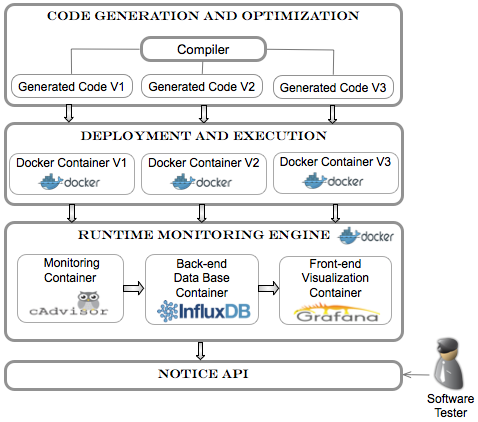
\includegraphics[width=1.\linewidth]{Ressources/genecoApproach.png}
	\caption{Overview of the Docker-based testing architecture}
\end{figure}


Our testing infrastructure will run different jobs within Docker containers. First, we generate and run different versions of code using our target compiler. To do so, we run multiple instances of our preconfigured Docker image that corresponds to specific code generator (e.g, GCC compiler). Each container will execute a specific job. For our case, a job represents a program compiled with new optimization sequence generated by NS. In the meanwhile, we start our runtime testing components (e.g., cAdvisor, InfluxDB and Grafana). The monitoring component collects usage statistics of all running containers and save them at runtime in the time series database component. The visualization component comes later to allow end users to define performance metrics and draw up charts.


\section{Evaluation}
So far, we have presented a sound procedure and automated component-based framework for extracting non-functional properties of generated code. In this section, we evaluate the implementation of our approach by explaining the design of our empirical study; the research questions we set out to answer and different methods we used to answer these questions. The experimental material is available for replication purposes at~\cite{mboussaa}.

\subsection{Research questions}
Our experiments aim at answering the following research questions:

\textbf{RQ1: Mono-objective SBSE Validation.} 
\textit{How does the proposed diversity-based exploration of optimization sequences perform compared to other mono-objective algorithms in terms of memory and CPU consumption, execution time, etc.?} 
 

\textbf{RQ2: Sensitivity.} 
\textit{How sensitive are input programs to compiler optimization options?}


\textbf{RQ3: Impact of optimizations on resource consumption.} 
\textit{How compiler optimizations impact on the non-functional properties of generated programs?}


\textbf{RQ4: Trade-offs between non-functional properties.} 
\textit{How can multi-objective approaches be useful to find trade-offs between non-functional properties?}

To answer these questions, we conduct several experiments using NOTICE to validate our global approach for non-functional testing of compilers using system containers.
 

\subsection{Experimental Setup}
\subsubsection{Programs Used in the Empirical Study}
To explore the impact of compiler optimizations a set of input programs are needed. 
To do so, we use a random C program generator called Csmith~\cite{yang2011finding}.
Csmith is a tool that can generate random C programs that statically and dynamically conform to the C99 standard. It has been widely used to perform functional testing of compilers~\cite{chen2016empirical,le2014compiler,nagai2013scaling} but not the case for checking non-functional requirements, that is why we choose Csmith as program generator. Csmith can generate C programs that utilize a much wider range of C features including complex control flow and data structures such as pointers, arrays, and structs. Csmith programs come with their test suites that explore the structure of generated programs. 
Authors argue that Csmith is an effective bug-finding tool because it generates tests that explore atypical combinations of C language features. They also argue that larger programs are more effective for functional testing. Thus, we run Csmith for 24 hours and gathered the largest generated programs. We depicted 111 C programs with an average number of source lines of 12K. 10 programs are used as training set for RQ1, 100 other programs to answer RQ2 and 1 last program to run RQ3 experiment.
Selected Csmith programs are described in more details at~\cite{mboussaa}.
%Moreover, we run experiments on commonly used benchmarks in iterative compilation named Collective Benchmark (Cbench)~\cite{fursin2009collective}. It is a collection of open-source sequential programs in C, targeting specific areas of the embedded market. It comes with multiple datasets assembled by the community to enable realistic benchmarking and research on program and architecture optimization. Cbench contains more than 20 C programs. 

\iffalse
\begin{table}[h]
	\begin{center}
		\begin{tabular}{|c|c|p{3.9cm}|}
			\hline
			\textbf{Program} & \textbf{Source lines} & \textbf{Description}\\
			\hline
			automative\_susan\_s & 1376 & Image recognition package\\
			\hline
			bzip2e & 5125 & Compress any file
			source code \\
			\hline
			bzip2d & 5125 & Decompress zipped files \\
			\hline
			office\_rsynth & 4111 & Text to speech program produced by integrating various pieces of code\\
			\hline
			consumer\_tiffmedian& 15870 & Apply the median cut algorithm to data in a TIFF file
			\\
			
			\hline
			consumer\_tiffdither& 15399 & Convert a greyscale image to bilevel using dithering
			\\
			\hline
			
		\end{tabular}
		
	\end{center}
	\caption {Description of selected benchmark programs}
\end{table}
\fi
\subsubsection{Parameters Tuning}
%Our experiments use the classical NS algorithm, where we evolve a set of optimization sequences through generations.
An important aspect for meta-heuristic search algorithms lies in the parameters tuning and selection, which is necessary to ensure not only fair comparison, but also for potential replication.
NOTICE implements 3 mono-objective search algorithms (NS, RS and GA~\cite{cooper2002adaptive}) and 3 multi-objective optimizations (NS, RS and NSGA-II~\cite{deb2002fast}). Each initial population/solution of different algorithms is completely random. The stopping criterion is when the maximum number of fitness evaluations is reached.
The resulting parameter values are listed in Table 2. The same parameter settings are applied to all algorithms under comparison.

NS, which is our main concern in this work, is implemented as described in Section 3. During the evolutionary process, each solution is evaluated using the novelty metric. Novelty is calculated for each solution by taking the mean of its 15 nearest optimization sequences in terms of similarity (considering all sequences in the current population and in the archive). Initially, the archive is empty. Novelty distance is normalized in the range [0-100].
Then, to create next populations, an elite of the 10 most novel organisms is copied unchanged, after which the rest of the new population is created by tournament selection according to novelty (tournament size = 2). Standard genetic programming crossover and mutation operators are applied to these novel sequences in order to produce offspring individuals and fulfill the next population (crossover = 0.5, mutation = 0.1).
In the meanwhile, individuals that get a score higher than 30 (threshold T), they are automatically added to the archive as well. 
In fact, this threshold is dynamic. Every 200 evaluations, we check how many individuals have been copied into the archive. If this number is below 3, the threshold is increased by multiplying it by 0.95, whereas if solutions added to archive are above 3, the threshold is decreased by multiplying it by 1.05. 
Moreover, as the size of the archive grows, the nearest-neighbor calculation that determines the novelty scores for individuals becomes more computationally demanding. So, to avoid having low accuracy of novelty, we choose to bound the size of the archive (archive size is 500). Hence, it follows a first-in first-out data structure which means that when a new solution gets added, the oldest solution in the novelty archive will be discarded. Thus, we ensure individual diversity by removing old sequences that may no longer be reachable from the current population.

Algorithm parameters were tuned individually in preliminary experiments. For each parameter, a set of values was tested. The parameter values chosen are the mostly used in the literature~\cite{lehman2008exploiting}. The value that yielded the highest performance score was chosen.  

\begin{table}
	\caption{Algorithm parameters}
	\begin{tabular}{| l |l| l |l| }\hline
		\textbf{Parameter} & \textbf{Value} & \textbf{Parameter} & \textbf{Value} \\	\hhline{|=|=|=|=|}	
		Novelty nearest-k  & 15 &  Tournament size & 2\\ 
		Novelty threshold & 30 &  Mutation prob. & 0.1\\  
		Max archive size & 500 &  Crossover & 0.5  \\  
		Population size & 50 &  Nb generations &  100 \\  
		Individual length & 76 & Elitism & 10  \\ 
		Scaling archive prob. & 0.05 & Solutions added to archive & 3  \\ 	\hline
	\end{tabular}
\end{table}

\subsubsection{Evaluation Metrics Used}

For mono-objective algorithms, we use to evaluate solutions using the following metrics:

-\textit{Memory Consumption Reduction (MR)}: corresponds to the percentage ratio of memory usage reduction of running container over the baseline. The baseline in our experiments is O0 level, which means non-optimized code. Larger values for this metric mean better performance. Memory usage is measured in bytes.

-\textit{CPU Consumption Reduction (CR)}: corresponds to the percentage ratio of CPU usage reduction over the baseline. Larger values for this metric mean better performance. The CPU consumption is measured in seconds, as the CPU time.

-\textit{Speedup (S)}: corresponds to the percentage improvement in speed of execution of an optimized code compared to the execution time of baseline version. Programs execution time is measured in seconds.


When comparing two mono-objective algorithms, it is usual to compare their best solutions found so far during the optimization process. However, this is not applicable when comparing two multi-objective evolutionary algorithms since each of them gives as output a set of non-dominated (Pareto equivalent) solutions. For this reason, we use performance indicator to compare multi-objective algorithms.
Thus, for multi-objective algorithms we use to evaluate solutions using the following metric:

-\textit{Hypervolume (HV)}: corresponds to the proportion of objective space that is dominated by the Pareto front approximation returned by the algorithm and delimited by a reference point. The HV reference point is the point obtained by taking the maximum value observed. Thus, the HV metric can be computed as the area between the Pareto frontier and the HV reference point. Larger values for this metric mean better performance. The most interesting features of this indicator are its Pareto dominance compliance and its ability to capture both convergence and diversity~\cite{deb2001multi}. 

\subsubsection{Setting up infrastructure}
To answer the previous research questions, we configure NOTICE to run different experiments. Figure 4 shows a big picture of the testing and monitoring infrastructure considered in these experiments. 
First, a meta-heuristic (mono or multi-objective) is applied to generate specific optimization sequences for the GCC compiler (step 1). During all experiments, we use GCC 4.8.4, as it is introduced in the motivation section, although it is possible to choose another compiler version using NOTICE since the process of optimizations extraction is done automatically. 
Then, we apply the generated optimization sequences to the input program under test and deploy the output binary within a new instance of our preconfigured docker image (step 2). While executing the optimized code inside the container, we collect runtime performance data (step 4) and record it in a new time-series database using our InfluxDB back-end container (step 5). Next, NOTICE accesses remotely to stored data in InfluxDB using REST API calls and assigns new performance values to the current solution (step 6). The choice of performance metrics depends on experiment objectives (Memory improvement, speedup, etc.).
\begin{figure}[h]
	\centering
	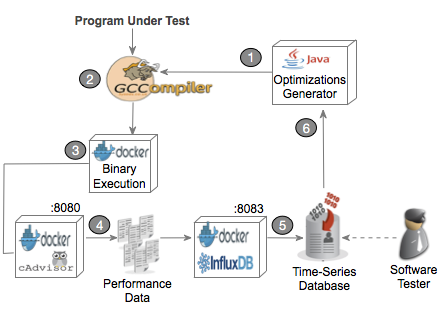
\includegraphics[width=0.9\linewidth]{Ressources/infraup.png}
	\caption{NOTICE experimental infrastructure}
\end{figure}

To obtain comparable and reproducible results, we use the same hardware across all experiments: an AMD A10-7700K APU Radeon(TM) R7 Graphics processor with 4 CPU cores (2.0 GHz), running Linux with a 64 bit kernel and 16 GB of system memory.



\section{Related Work}
Our work is related to iterative compilation research field.
The basic idea of iterative compilation is to explore the compiler optimization space by measuring the impact of optimizations on software performance.
Several research efforts have investigated this optimization problem using search-based techniques (SBSE) to guide the search towards relevant optimizations regrading performance, energy consumption, code size, compilation time, etc. Experimental results have been usually compared to standard compiler optimization levels.  
The vast majority of the work on iterative compilation focuses on increasing the speedup of new optimized code compared to standard compiler optimization levels~\cite{almagor2004finding,hoste2008cole,pan2006fast,pallister2015identifying,chen2012deconstructing,martins2014exploration,lin2008automatic,martinez2014multi}.
It has been proven that optimizations are highly dependent on target platform and input program. 
Compared to our proposal, none of the previous work has studied the impact of compiler optimizations on resource usage. In this work, we rather focus on compiler optimizations related to resource consumption, while bearing in mind the performance improvement.

Novelty Search has never been applied in the field of iterative compilation. Our work presents the first attempt to introduce diversity in the compiler optimization problem. 
The idea of NS has been introduced by Lehman et al.~\cite{lehman2008exploiting}. It has been often evaluated in deceptive tasks and especially applied to evolutionary robotics~\cite{risi2010evolving,krvcah2012solving} (in the context of neuroevolution). 
NS can be easily adapted to different research fields. In a previous work~\cite{boussaa2015novelty}, we have adapted the general idea of NS to the test data generation problem where novelty score was calculated as the Manhattan distance between the different vectors representing the test data. The evaluation metric of generated test suites is the structural coverage of code.
In this paper, the evaluation metric represents the non-functional improvements and we are calculating the novelty score as the symmetric difference between optimization sequences. 

For multi-objective optimizations, we are not the first to address this problem. New approaches have emerged recently to find trade-offs between non-functional properties~\cite{hoste2008cole,martinez2014multi,lokuciejewski2010multi}. Hoste et al.~\cite{hoste2008cole}, which is the most related work to our proposal, propose COLE, an automated tool for optimization generation using a multi-objective approach namely SPEA2. In their work, they try to find Pareto optimal optimization levels that present a trade-off between execution and compilation time of generated code. Their experimental results show that the obtained optimization sequences perform better than standard GCC optimization levels. NOTICE provides also a fully automated approach to extract non-functional properties. However, NOTICE differs from COLE because first, our proposed container-based infrastructure is more generic and can be adapted to other case studies (i.e., compilers, code generators, etc.). Second, we provide facilities to compiler users to extract resource usage metrics using our monitoring components. Finally, our empirical study investigates different trade-offs compared to previous work in iterative compilation.



%For code generators testing, Stuermer et al.~\cite{stuermer2007systematic} present a systematic test approach for model-based code generators. They investigate the impact of optimization rules for model-based code generation by comparing the output of the code execution with the output of the model execution. 
%If these outputs are equivalent, it is assumed that the code generator works as expected. 
%They evaluate the effectiveness of this approach by means of testing optimizations performed by the TargetLink code generator. 
%They have used Simulink as a simulation environment of models. 
%In our approach, we provide a component-based infrastructure to compare non-functional properties of generated code rather than functional ones. 


\section{Conclusion and Future Work}
%We present an automated approach for automatic extraction of non-functional properties of generated code.
Modern compilers come with huge number of optimizations, making complicated for compiler users to find best optimization sequences. Furthermore, auto-tuning compilers to meet user requirements is a difficult task since optimizations may depend on different properties (e.g., platform architecture, software programs, target compiler, optimization objective, etc.).
Hence, compiler users merely use standard optimization levels (O1, O2, O3 and Ofast) to enhance code quality without taking too much care about the impact of optimizations on system resources.

In this paper, we have introduced first a novel formulation of the compiler optimization problem based on Novelty Search. The idea of this approach is to drive the search for best optimizations towards novelty. Our work presents the first attempt to introduce diversity in iterative compilation. Experiments have shown that Novelty Search can be easily applied to mono and multi-objective search problems. In addition, we have reported the results of an empirical study of our approach compared to different state-of-the-art approaches, and the results obtained have provided evidence to support the claim that Novelty Search is able to generate effective optimizations.

Second, we have presented an automated tool for automatic extraction of non-functional properties of optimized code, called NOTICE. NOTICE applies different heuristics (including Novelty Search) and performs non-functional testing of compilers through the monitoring of generated code in a controlled sand-boxing environment. In fact, NOTICE uses a set of micro-services to provide a fine-grained understanding of optimization effects on resource consumption. 
We evaluated the effectiveness of our approach by verifying the optimizations performed by GCC compiler. 
%Then, we studied the impact of optimizations on memory consumption and execution time across two case studies. 
Results showed that our approach is able to automatically extract information about memory and CPU consumption. We were also able to find better optimization sequences than standard GCC optimization levels.

As a future work, we plan to explore more trade-offs among resource usage metrics \eg, the correlation between CPU consumption and platform architectures. 
We also intend to provide more facilities to NOTICE users in order to test optimizations performed by modern compilers such as Clang, LLVM, etc.
Finally, NOTICE can be easily adapted and integrated to new case studies. As an example, we would inspect the behavior of model-based code generators since different optimizations can be performed to generate code from models~\cite{stuermer2007systematic}. Thus, we aim to use the same approach to find non-functional issues regarding code generation processes.








\section*{Acknowledgment}

This work was funded by the European Union Seventh Framework Programme (FP7/2007-2013) under grant agreement n611337, HEADS project (www.heads-project.eu)




% conference papers do not normally have an appendix


% use section* for acknowledgement
%\section*{Acknowledgment}


%The authors would like to thank...





% trigger a \newpage just before the given reference
% number - used to balance the columns on the last page
% adjust value as needed - may need to be readjusted if
% the document is modified later
%\IEEEtriggeratref{8}
% The "triggered" command can be changed if desired:
%\IEEEtriggercmd{\enlargethispage{-5in}}

% references section

% can use a bibliography generated by BibTeX as a .bbl file
% BibTeX documentation can be easily obtained at:
% http://www.ctan.org/tex-archive/biblio/bibtex/contrib/doc/
% The IEEEtran BibTeX style support page is at:
% http://www.michaelshell.org/tex/ieeetran/bibtex/
%\bibliographystyle{IEEEtran}
% argument is your BibTeX string definitions and bibliography database(s)
%\bibliography{IEEEabrv,../bib/paper}
%
% <OR> manually copy in the resultant .bbl file
% set second argument of \begin to the number of references
% (used to reserve space for the reference number labels box)

\bibliographystyle{IEEEtran}
\bibliography{ref}
	\cleardoublepage
	\cleardoublepage
\section{Evaluation}
In this section, we evaluate the implementation of our approach across two case studies. These experiments aim at answering the following research questions:

\textbf{RQ1:} How do standard GCC optimization levels influence on the resource consumption of generated programs?
To answer this question, we apply standard optimization options to FFmpeg library. Then, we evaluate the memory footprint and execution time of running FFmpeg command lines and we compare the results. The goal of this initial experiment is to
provide an understanding of the performance of generated code by GCC.

\textbf{RQ2:} To what extent can the proposed diversity-based exploration of optimization options impact the resource consumption of generated programs?
In a second experiment, we assess our NS approach for automatic optimization sequences generation by comparing the results found when applying standard optimization sequences to new results provided by our approach. The experimental results show that our novelty-based approach can produce optimization sequences with good performance and less resource consumption
than standard optimization levels in GCC. In this experiment, we study the correlation between execution time and memory consumption of generated code.

These two case studies  also enable to validate the global approach for non functional testing of code generators using system containers. 



\subsection{Case Study 1: FFmpeg}
In the first experiment, we set up our infrastructure for testing and monitoring of generated code. In this part, we compile the FFmpeg library using standard GCC optimizations(O1, O2, O3, Ofast) and we study the impact of these optimizations on memory consumption and execution time using our Docker-based infrastructure.

\subsubsection{FFmpeg: Multimedia Encoding Library}
FFmpeg\footnote{https://www.ffmpeg.org/} is a complete, cross-platform solution to record, convert, and stream audio and video. It is a very fast video and audio converter. It includes libraries of audio/video codecs and a command-line program for transcoding multimedia files. FFmpeg allows different types of multimedia conversion and that depends on the input and output format (video, audio, subtitle, attachment, data). Video/audio processing with FFmpeg usually need high-performance requirements and an important amount of resources in term of memory usage. So, testing GCC on top of this library is very interesting in order to compare resource usage profiles. 
\subsubsection{Docker-based Infrastructure for Monitoring FFmpeg Containers}


The goal of this experiment is to compile FFmpeg with standard GCC optimization options and run FFmpeg command examples on top of different versions in order to compare the memory usage profiles and execution time of different variants using our test architecture. An overview of the different components involved in testing and monitoring of FFmpeg containers is shown in Figure 2. 
First, we compile FFmpeg library with different optimization options  (O0, O1, O2, O3 and Ofast) in order to produce 5 variants of FFmpeg. This is done within Docker containers. We configure each container to install FFmpeg with a specific configuration and we upload all FFmpeg images in Docker Hub\footnote{https://hub.docker.com/}.
Docker Hub is a cloud-based registry service for building and shipping application or service containers. We use it for building, saving, and managing all our Docker images.

Afterwards, we execute the same stressload (FFmpeg examples) within each FFmpeg instance container. We choose 15 FFmpeg command examples that cover multiple domains\footnote{http://goo.gl/11VLYM} like video conversion, sound extraction, encoding file for iPod or PSP, etc. This list of examples is saved in a script file that should be executed later within FFmpeg containers. The media files needed for encoding are saved in a shared repository. In Docker environment, we call this repository the “Data Volume”. A data volume is a specially-designated directory within containers that share data with the host machine. Data is persistent and independent of container's life cycle. So, when we run FFmpeg containers we provide a shared volume with the host machine (where the media files are located). As well, the list of FFmpeg commands to execute is mounted in this volume so that, we can execute the same workload each time we run a new container.
Before running FFmepg workload on different containers, we run monitoring components (cAdvisor, InfluxDB and Grafana) to start gathering usage statistics.
In fact, in this experiment, we choose to gather statistics about memory consumption and execution time of different containers. 

To obtain comparable and reproducible results, we use the same hardware across all experiments: an AMD A10-7700K APU Radeon(TM) R7 Graphics processor with 4 CPU cores (2.0 GHz), running Linux with a 64 bit kernel and 16 GB of system memory.

\subsubsection{Experimental Results}
\begin{figure}[!t]
	\centering
	\includegraphics[width=1.\linewidth]{Ressources/infra_ffmpeg.png}
	\caption{Overview of the different components involved in testing and monitoring of FFmpeg containers}
\end{figure}


\begin{figure}[tbh]
	\includegraphics[width=1\linewidth]{Ressources/infra_stats.png}
	\caption{Snapshot of runtime memory consumption profiles of FFmpeg containers compiled with O0 (no optimization) and O3 options}
	%		\label{AAA}
\end{figure}

In this first part of experiments with FFmpeg, we compare a zero-level optimization container (FFmpeg-O0) with a high-level optimization one (FFmpeg-O3) in order to study the impact of optimizations on memory usage and execution time. Figure 3 shows runtime statistics of running two FFmpeg containers O0 and O3 with the same input workload. This chart depicts a snapshot of our visualization component web UI. It presents the memory usage profiles of two components (FFmpeg O0 and O3) started in the same time and running in parallel. Visually, we can see that the execution time of O3 (yellow) is faster than O0 (green) since O3 execution ended before O0. However, we can see that memory usage remains higher than O0 from the beginning to the end of running FFmpeg examples. 

To better understand the resource usage of optimized code, we run the same experiment for all FFmpeg containers and we collect the same metrics. Figure 4 presents a comparison of average memory usage and execution time of FFmpeg containers compiled with all standard GCC optimization options. We notice that the memory usage increases as soon as we apply more aggressive optimization. However, when we apply higher optimization level, we clearly improve the execution time compared to O0. For example, O3 and Ofast have the highest memory consumption (100 MBytes more than O0) and best execution time (speedup around 1.8) which can be inconvenient for systems with limited resources.

This results explain that optimizing for execution time (for the case of FFmpeg) is not always efficient regarding memory usage and unfortunately, optimizations may influence negatively the system resources.
\begin{figure}[hbt]
	\centering
	\includegraphics[width=1\linewidth]{Ressources/infra_ffmpeg_plot1.png}
	\caption{Comparison of average memory consumption and execution time of FFmpeg containers compiled with standard GCC optimization options}
\end{figure}


\subsection{Case Study 2: Novelty-based Exploration of Optimization Sequences}
In this second case study, we assess the performance of GCC compiler across different benchmark programs. The goal of this experiment is to show that our approach for exploring the search space of optimizations is able to generate efficient code that yields to less resource consumption than GCC default optimizations.
\subsubsection{Setting Up Infrastructure}
\begin{figure}[b]
	\centering
	\includegraphics[scale=0.50]{Ressources/infra_novelty.png}
	\caption{Overall process of monitoring code generated by GCC}
	
%	\vspace*{-5cm}
	
\end{figure}
For this experiment, we keep the same architecture settings as first case study. However, we provide a more generalized approach for automatic testing of code generators using system containers. So, starting from a list of optimizations defined by the user, an input program and a specific target compiler, we are able to execute and monitor optimized code. Figure 5 shows more details about this process. First, our novelty-based test sequences generator generates a huge amount of diverse optimizations. We compile an input program with these generated sequences using GCC. Then, we execute produced binaries sequentially within isolated Docker containers (Docker image with GCC version 4.8.4 installed above). We keep the same monitoring chain to gather resource usage of running containers. This process is repeated until the end of generated sequences. Finally, end-users (testers) can access to resource consumption statistics through InfluxDB or Grafana Web UI to compare the impact of optimizations on resource consumption. In this example too, we choose to focus on studying the trade-off memory usage/execution time. 
\subsubsection{Benchmark programs}
To explore the impact of compiler optimizations a set of input programs are needed. We run experiments on commonly used benchmarks named Collective Benchmark (cBench)~\cite{fursin2009collective}. It is a collection of open-source sequential programs in C targeting specific areas of the embedded market. It comes with multiple datasets assembled by the community to enable realistic benchmarking and research on program and architecture optimization. cBench contains more than 20 C programs. The following table describes programs that we have selected from this benchmark to evaluate our approach.
\begin{table}[h]
	\begin{center}
		\begin{tabular}{|c|c|p{3.9cm}|}
			\hline
			\textbf{Program} & \textbf{Source lines} & \textbf{Description}\\
			\hline
			automative\_susan\_s & 1376 & Image recognition package\\
			\hline
			bzip2e & 5125 & Compress any file
			source code \\
			\hline
			bzip2d & 5125 & Decompress zipped files \\
			\hline
			office\_rsynth & 4111 & Text to speech program produced by integrating various pieces of code\\
			\hline
			consumer\_tiffmedian& 15870 & Apply the median cut algorithm to data in a TIFF file
			\\
			
			\hline
			 consumer\_tiffdither& 15399 & Convert a greyscale image to bilevel using dithering
			 \\
			\hline
			
		\end{tabular}
		
	\end{center}
	\caption {Description of selected benchmark programs}
\end{table}
\subsubsection{Novelty Parameters}
%Our experiments use the classical NS algorithm, where we evolve a set of optimization sequences through generations.
NS is implemented as described in Section 3.
The first step in the process of selection is to evaluate each individual and compute its novelty score. Novelty is calculated for each organism by taking the mean of its 15 lowest dissimilar optimization sequences (considering all sequences in the current population and in the archive). 
Then, to create next populations, an elite of the 10 most novel organisms is copied unchanged, after which the rest of the new population is created by tournament selection according to novelty. Standard genetic programming crossover and mutation operators are applied to these novel sequences in order to produce offspring individuals and fulfill the next population.
In the meanwhile, individuals that get a score higher than the threshold T they are automatically added to the archive as well. 
In fact, this threshold is dynamic. Every 150 evaluations, we check how many individuals have been copied into the archive. If this number is below 3, the threshold is increased by multiplying it by 0.95, whereas if solutions added to archive are above 3, the threshold is decreased by multiplying it by 1.05. 
Moreover, as the size of the archive grows, the nearest-neighbor calculations that determine the novelty scores for individuals become more computationally demanding. So to avoid having low accuracy of novelty, we choose to bound the size of the archive. Hence, it follows a first-in first-out data structure which means that when a new solution gets added, the oldest solution in the novelty archive will be discarded. Thus, we ensure individuals diversity by removing old sequences that may no longer be reachable from the current population.

The parameters of the algorithm were tuned individually in preliminary experiments. For each parameter, a set of values was tested. The parameter values chosen are the mostly used in the literature~\cite{lehman2008exploiting}. The value that yielded the highest performance scores was chosen. The resulting parameter values are listed in Table 4.
\begin{table}
		\caption{Parameters of NS algorithm}
		\begin{tabular}{ l l || l l }
			Parameter & Value & Parameter & Value \\	\hline
			Novelty nearest-k  & 15 &  Tournament size & 2\\ 
			Add archive prob. & 30 &  Mutation prob. & 0.1\\  
			Max archive size & 500 &  Crossover & 0.5  \\  
			Population size & 100 &  Nb generations &  100 \\  
			Individual length & 76 & Elitism & 10  \\ 
			Scaling archive prob. & 0.05 & Solutions added to archive & 3  \\ 
		\end{tabular}
\end{table}

\subsubsection{Experimental results}

The goal of this experiment is to compare novelty-based generated sequences to standard GCC optimizations in term of memory consumption. Figure 6 shows this comparison across different benchmark programs. It presents the percentage of saved memory of standard and novelty optimizations over O0 level (no optimization applied).
 
\begin{figure}[!ht]
	\centering
	\includegraphics[width=1.\linewidth]{Ressources/infra_novelty_stat3.png}
	\caption{Evaluating the amount of saved memory after applying standard optimization options compared to best generated optimization using NS}
\end{figure}

For NS, we select the best sequence that reduces the memory consumption and we compare it to the memory footprint of O0, O1, O2, O3 and Ofast versions. The results show clearly that NS outperforms standard optimizations for all benchmark programs. Using NS, we are able to reach a maximum memory consumption reduction of almost 26\% for the case rsynth program against a maximum of 18\% reduction using Ofast option. We remark as well that the impact of applying standard optimizations on memory consumption for each program differs from one program to another. Using O1 for bzip2e and O2, O3 for tiffmedian can even increase the memory consumption by almost 13 \% (like the FFmpeg experiments). This agrees to the idea that standard optimizations does not produce always the same impact results on resource consumption and may be highly dependent on the benchmark and the source code they have been tested on. Our approach can clearly provide an alternative to catch most relevant optimization sequence regarding resource consumptions.

To study the correlation between execution time and memory consumption of running programs, we present in Figure 7 an evaluation of the speedup. We compare the speedup (according to O0) of the best optimization sequences by NS (gathered in Figure 6) with standard optimization options. 
The first observation is that optimizations yield to high level of speedup for all benchmark programs (between 1.5 and 4.3).
The second observation we can make is that different optimizations do not differ too much in term of execution time. We  distinguish that Ofast is slightly more efficient for all programs and NS sequence has almost the same speedup as Ofast. 
The results of this experiments shows that optimizing for memory usage using NS does not affect programs execution time and we demonstrate that we can find optimizations that reduce memory usage while guaranteeing program performance.
\begin{figure}[!ht]
	\centering
	\includegraphics[width=1.\linewidth]{Ressources/infra_novelty_stat2.png}
	\caption{Evaluating the speedup after applying standard optimization options compared to best generated optimization using NS}
\end{figure}



% that's all folks
\end{document}